\section{First data set}

The aim of this task is to find a suitable distribution for \emph{Body Mass Index} (\textbf{BMI}) data for boys of
a particular age.  The data is from the study \citetitle{Fredriks:2000} by \citeauthor{Fredriks:2000}
\citeyear{Fredriks:2000} \cite{Fredriks:2000}.

BMI is a number calculated from a person's height in meters and weight in kilograms:
\begin{equation}
  BMI = \frac{kg}{m^2}
\end{equation}

The data set has two columns \verb|age| and \verb|bmi|.  Both column contain positive real values.

\begin{table}[!ht]
\begin{verbatim}
      age              bmi       
 Min.   : 0.030   Min.   :11.17  
 1st Qu.: 1.863   1st Qu.:15.96  
 Median :10.450   Median :17.45  
 Mean   : 9.291   Mean   :18.03  
 3rd Qu.:15.130   3rd Qu.:19.60  
 Max.   :21.700   Max.   :35.42  
\end{verbatim}
\caption {Summary information on the \texttt{dbbmi} data}
\end{table}


\subsection{Distributions Under Consideration}

We are asked to interpret the bmi information of subjects within a one year
age group.  From the summary information we are looking at, the response
variable of `bmi` is a continuous random variable.

As there is no definition of the upper bounds of a person's height or weight,
there's no natural justification to normalise the value of `bmi`, so we are
interested in families of continuous distributions over the positive real
range $R_Y = (0, \infty)$.

Although we are strictly bounded by zero, as a population ages and the average
weight increases, the distribution will shift to the right, and we may find that
shifted continuous distributions over the real range $R_Y =  (-\infty, \infty)$ will
also give good results.

Looking at the histogram, there is perhaps some sign of skew on the right of the distribution.
But more importantly we can see an excess extreme values at a BMI of $(26, 27)$ and
further outliers in $(30, 31)$ and $~35$, indicating a leptokurtic distribution.

\begin{figure}[H]
  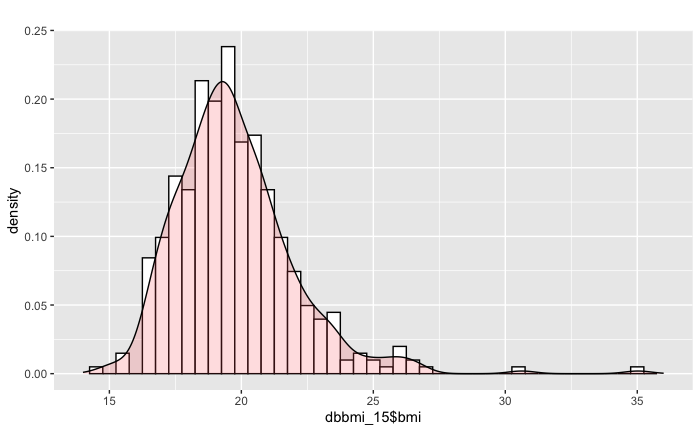
\includegraphics{q1_histogram_dbbmi_15.png}
  \caption{Histogram of BMI for 15 year old Dutch boys \cite{Fredriks:2000}}
\end{figure}
  
The initial intuition is that we will be at least considering, at least over the positive-real values,
a three-parameter distribution to model either skewness or kurtosis in
addition to location and scale.  If the data
requires both skewness and kurtosis, then a four-parameter distribution should give better
results.

\subsection{Selecting the Distribution}

The selected distribution is the \textbf{Exponential Gaussian:} \verb|exGAUS|.

As there are no explanatory variables, we can use \verb|GAMLSS| function \verb|fitDist|, which uses the
maximum likelihood and selected the best fitting distribution according to the GAIC \cite{Rigby:2019}.  It
fits all relevant parametric \verb|gamlss.family| distributions
to a single data vector, choosing the final marginal distributions with the lowest
Akaike Information Criteria (AIC) value with a penality of $k=2$.

The results for the best performing (lowest GAIC score) distributions are:

\begin{table}[!ht]
\begin{verbatim}
  exGAUS    BCPEo     BCPE     BCTo      BCT      ST5    BCCGo     BCCG      GB2 ...
1729.537 1729.731 1729.731 1729.992 1729.992 1730.401 1730.663 1730.663 1730.882 ...
\end{verbatim}
\caption {\texttt{fitDist} results for \texttt{dbbmi\_15\$bmi} data}
\end{table}

The distribution is a three-parameter distribution \verb|exGAUS|$(\mu, \sigma, \nu)$.  It combines features
of both the normal distribution and the exponential distributions, and captures tails that skew to one
side \cite{Rigby:2019}.  

\begin{figure}[H]
  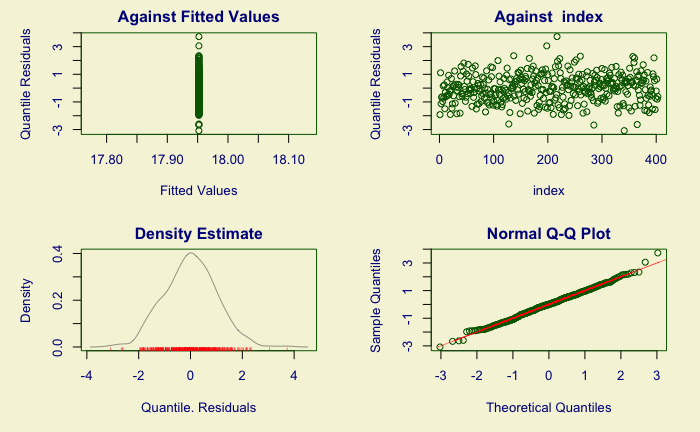
\includegraphics{q1_exgaus_plot.png}
  \caption{Fitted \texttt{exGAUS} distribution and \texttt{bmi} histogram}
\end{figure}


We can see

\begin{figure}[H]
  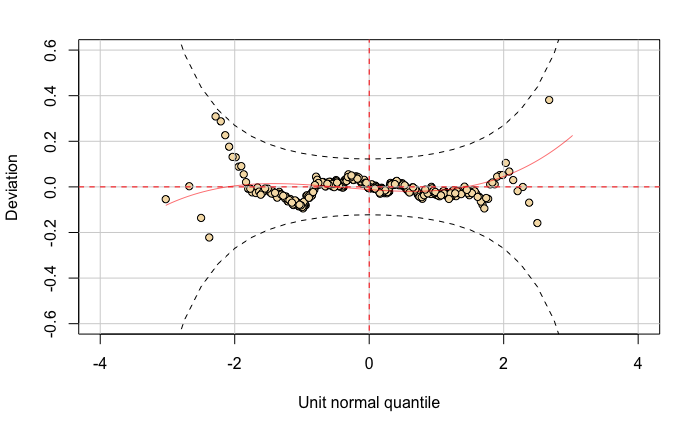
\includegraphics{q1_exgaus_wp.png}
  \caption{Fitted \texttt{exGAUS} distribution residuals' worm plot}
\end{figure}

\subsection{Interpreting the Fitted Distribution}

\begin{table}[H]
\begin{verbatim}
******************************************************************
Family:  c("exGAUS", "ex-Gaussian")

Call:  gamlss(formula = bmi ~ 1, family = "exGAUS", data = dbbmi_15)

Fitting method: RS()

------------------------------------------------------------------
Mu link function:  identity
Mu Coefficients:
            Estimate Std. Error t value Pr(>|t|)
(Intercept)  17.9521     0.1492   120.3   <2e-16 ***
---
Signif. codes:  0 ‘***’ 0.001 ‘**’ 0.01 ‘*’ 0.05 ‘.’ 0.1 ‘ ’ 1

------------------------------------------------------------------
Sigma link function:  log
Sigma Coefficients:
            Estimate Std. Error t value Pr(>|t|)
(Intercept)  0.24593    0.08047   3.056  0.00239 **
---
Signif. codes:  0 ‘***’ 0.001 ‘**’ 0.01 ‘*’ 0.05 ‘.’ 0.1 ‘ ’ 1

------------------------------------------------------------------
Nu link function:  log
Nu Coefficients:
            Estimate Std. Error t value Pr(>|t|)
(Intercept)  0.58625    0.09008   6.508 2.28e-10 ***
---
Signif. codes:  0 ‘***’ 0.001 ‘**’ 0.01 ‘*’ 0.05 ‘.’ 0.1 ‘ ’ 1

------------------------------------------------------------------
No. of observations in the fit:  403
Degrees of Freedom for the fit:  3
      Residual Deg. of Freedom:  400
                      at cycle:  15

Global Deviance:     1723.537
            AIC:     1729.537
            SBC:     1741.534
******************************************************************
\end{verbatim}
\caption{Fitted coefficients and their standard errors for \texttt{exGAUS}}
\end{table}



Our fitted distribution can then be described as \verb|exGAUS|$(\mu=17.9521, \sigma=exp(0.24593), \nu=exp(0.58625))$,
with the following definitions\cite{Rigby:2019}:
\begin{itemize}
\item $\mu$: mean of the gaussian and hence the location shift parameter.
\item $\sigma$: std. deviation of the gaussian, but not the scaling parameter.
\item $\nu$: mean of the exponential.
\item $\alpha_1 = \sigma + \mu$: Scaling parameter.
\end{itemize}


\begin{figure}[H]
  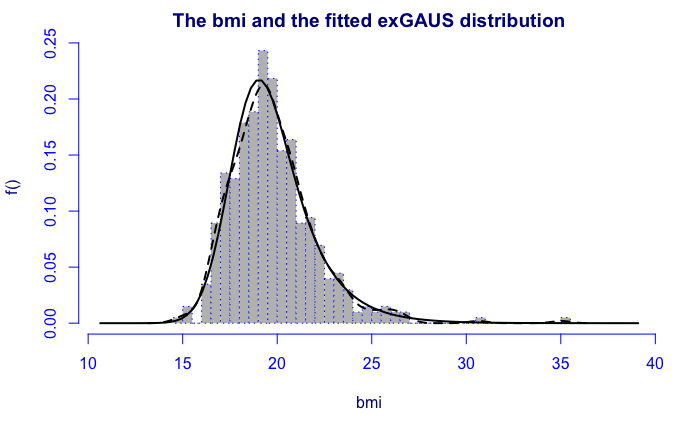
\includegraphics{q1_exgaus_fitted_hist.png}
  \caption{Fitted \texttt{exGAUS} distribution and \texttt{bmi} histogram}
\end{figure}

The fitted distribution matches the non-parametric density plot with reasonable accuracy,
with the notable exceptions on the right tail where we have already pointed out some extreme
values.

